\section{Mobile Antenna Limitations}
As the requirements for mobile antennas gets more and more strict, some trade off's need to be considered when designing an antenna.
The design constrains when designing small antennas for mobile phones is especially a trade off between size, bandwidth and efficiency, as illustrated in Figure \ref{fig:antenna_tradeoff}. 

The trade off relationship can be expressed as: 
\begin{align*}
  \frac{\Delta f}{f} \propto \frac{(a/ \lambda)^3}{\eta}
\end{align*}

This relationship expresses that it is very hard, if not impossible, to design a small antenna with excellent efficiency performance and a high bandwidth.
Therefor, when designing mobile antennas that requires high bandwidth and small antenna structures a trade off is needed to ensure that the antenna performs as required.

In the case of the project goal the antenna is desired to have a bandwidth from \SI{690}{MHz} to \SI{960}{MHz} in the low band and from \SI{1710}{MHz} to \SI{2650}{MHz} in the high band. Furthermore it needs to by very small with a ground clearance of \SI{5}{mm} and an efficiency above \SI{50}{\percent} in the entire bandwidth.

\begin{itemize}
\item $\lambda$ = Wavelength.
\item $\eta$ = Efficiency.
\item $\Delta f / f$ = Bandwidth.
\item $a^3$ = Antenna volume.
\end{itemize}

\begin{figure}[htbp]
  \centering
  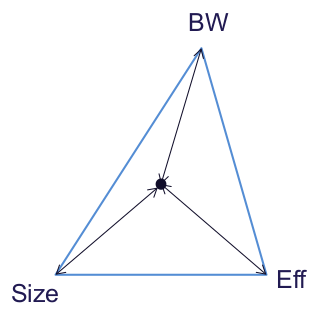
\includegraphics[scale=0.4]{img/analysis/antenna_limitations}
  \caption{Antenna design trade off's}
  \label{fig:antenna_tradeoff}
\end{figure}

\cite{hilbert2015tradeoff}